\section{Proposed Solution}
\label{sec:solution}

Considering the type of data we decided to solve the problem using Long Short Term Memory networks (LSTM) as it is a natural way to model problem. As a comparison, Multilayer perceptron was also implemented (MLP). From our analysis of the data, the input of our networks is the day of the year, page id and page views from the previous day or week.

\subsection{Long Short Term Memory networks}

Our implementation of the LSTM applies Backpropagation Through Time (BPTT) after each time step and uses batch normalization to avoid exploding gradients.
The model combines previous occurrences with data extracted from the current steps. So it receives page unique id, day from the start of the series and number of visits of the last day as input.

\begin{figure}[h!]
    \centering
    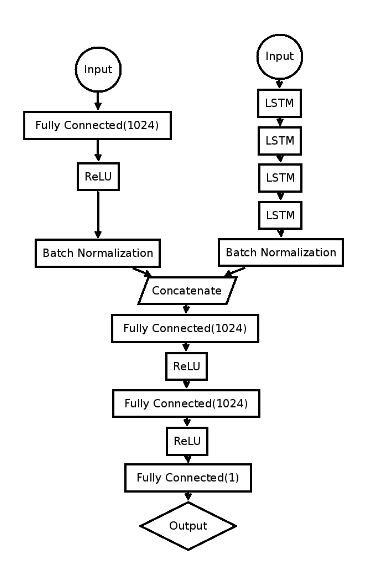
\includegraphics[width=\linewidth]{lstm.png}
    \caption{Observed Traffic and Traffic Trend from two different pages}
    \label{fig:analysis1}
\end{figure}


